% Options for packages loaded elsewhere
\PassOptionsToPackage{unicode}{hyperref}
\PassOptionsToPackage{hyphens}{url}
%
\documentclass[
]{article}
\usepackage{amsmath,amssymb}
\usepackage{iftex}
\ifPDFTeX
  \usepackage[T1]{fontenc}
  \usepackage[utf8]{inputenc}
  \usepackage{textcomp} % provide euro and other symbols
\else % if luatex or xetex
  \usepackage{unicode-math} % this also loads fontspec
  \defaultfontfeatures{Scale=MatchLowercase}
  \defaultfontfeatures[\rmfamily]{Ligatures=TeX,Scale=1}
\fi
\usepackage{lmodern}
\ifPDFTeX\else
  % xetex/luatex font selection
\fi
% Use upquote if available, for straight quotes in verbatim environments
\IfFileExists{upquote.sty}{\usepackage{upquote}}{}
\IfFileExists{microtype.sty}{% use microtype if available
  \usepackage[]{microtype}
  \UseMicrotypeSet[protrusion]{basicmath} % disable protrusion for tt fonts
}{}
\makeatletter
\@ifundefined{KOMAClassName}{% if non-KOMA class
  \IfFileExists{parskip.sty}{%
    \usepackage{parskip}
  }{% else
    \setlength{\parindent}{0pt}
    \setlength{\parskip}{6pt plus 2pt minus 1pt}}
}{% if KOMA class
  \KOMAoptions{parskip=half}}
\makeatother
\usepackage{xcolor}
\usepackage[margin=1in]{geometry}
\usepackage{graphicx}
\makeatletter
\def\maxwidth{\ifdim\Gin@nat@width>\linewidth\linewidth\else\Gin@nat@width\fi}
\def\maxheight{\ifdim\Gin@nat@height>\textheight\textheight\else\Gin@nat@height\fi}
\makeatother
% Scale images if necessary, so that they will not overflow the page
% margins by default, and it is still possible to overwrite the defaults
% using explicit options in \includegraphics[width, height, ...]{}
\setkeys{Gin}{width=\maxwidth,height=\maxheight,keepaspectratio}
% Set default figure placement to htbp
\makeatletter
\def\fps@figure{htbp}
\makeatother
\setlength{\emergencystretch}{3em} % prevent overfull lines
\providecommand{\tightlist}{%
  \setlength{\itemsep}{0pt}\setlength{\parskip}{0pt}}
\setcounter{secnumdepth}{-\maxdimen} % remove section numbering
\ifLuaTeX
  \usepackage{selnolig}  % disable illegal ligatures
\fi
\IfFileExists{bookmark.sty}{\usepackage{bookmark}}{\usepackage{hyperref}}
\IfFileExists{xurl.sty}{\usepackage{xurl}}{} % add URL line breaks if available
\urlstyle{same}
\hypersetup{
  pdftitle={Tvyal Newsletter},
  pdfauthor={Aghasi Tavadyan},
  hidelinks,
  pdfcreator={LaTeX via pandoc}}

\title{Tvyal Newsletter}
\author{Aghasi Tavadyan}
\date{2023-11-21}

\begin{document}
\maketitle

\textbf{\emph{English summary below.}}

Հարգելի գործընկեր,

Հուսով եմ լավ եք: Ներկայացնում եմ անցած շաբաթվա վերլուծությունները և
աշխատանքները.

\begin{enumerate}
\def\labelenumi{\arabic{enumi}.}
\tightlist
\item
  Բենզինի գնի թանկացման պատճառները
\item
  ԶԼՄ հաղորդագրություններ
\item
  Սպասում եմ ձեզ իմ սթրիմին
\item
  English summary
\end{enumerate}

\hypertarget{ux562ux565ux576ux566ux56bux576ux56b-ux563ux576ux56b-ux569ux561ux576ux56fux561ux581ux574ux561ux576-ux57aux561ux57fux573ux561ux57cux576ux565ux580ux568}{%
\subsection{1. Բենզինի գնի թանկացման
պատճառները}\label{ux562ux565ux576ux566ux56bux576ux56b-ux563ux576ux56b-ux569ux561ux576ux56fux561ux581ux574ux561ux576-ux57aux561ux57fux573ux561ux57cux576ux565ux580ux568}}

Այս շաբաթվա հետազոտությունը անելու համար օգտվել ենք հետևյալ
աղբյուրներից․

\begin{itemize}
\tightlist
\item
  Բենզինի և դիզելային վառելիքի գնի օրական տվյալների, ձևավորված
  \href{https://img.youtube.com/vi/tV15O3Ilrc8/maxresdefault.jpg}{1in.am
  Յութուբյան ալիքի տեսանյութերի նկարներից}
\item
  Վառելիքի թանկացման ամսական տվյալների բազան ըստ
  \href{https://www.armstat.am/am/?nid=82\&id=2611}{ՍԳԻ սկսած 2017թ․}
\item
  վառելիքի ներմուծման ամսական տվյալների բազան ըստ 6-նիշ արտաքին
  տնտեսական գործունեության ծածկագրերի և պետությունների
\end{itemize}

Բոլոր տվյալների բազաները և գծապատկերների կոդը առկա է իմ
\href{https://github.com/tavad/tvyal_newsletter}{Github-ում}

\begin{center}\rule{0.5\linewidth}{0.5pt}\end{center}

Նախ ուսումնասիրենք բենզինի գինը տարածաշրջանի այն երկրներում, որոնք
հիմնականում համարվում են նավթամթերք ներմուծող պետություն։ Նշեմ, որ
Հայաստանում համեմատած մեր հարևանների և ԵԱՏՄ երկրների բենզինի գինը
ամենաբարձրն է։ Սակայն սրա պատճառները հիմնականում տրանսպորտային ծախսերն
են և այն հանգամանքը, որ Հայաստանը նավթամթերք արտադրող պետություն չէ։ ՀՀ
դրամով հաշվարկված այս պահին, Վրաստանում բենզինի գինը կազմում է մոտ 500
դրամ։

\textbf{Գծապատկեր 1.} Բենզինի միջին գնիը Հայաստանում և տարածաշրջանի
բանզին ներմուծող այլ պետություններում

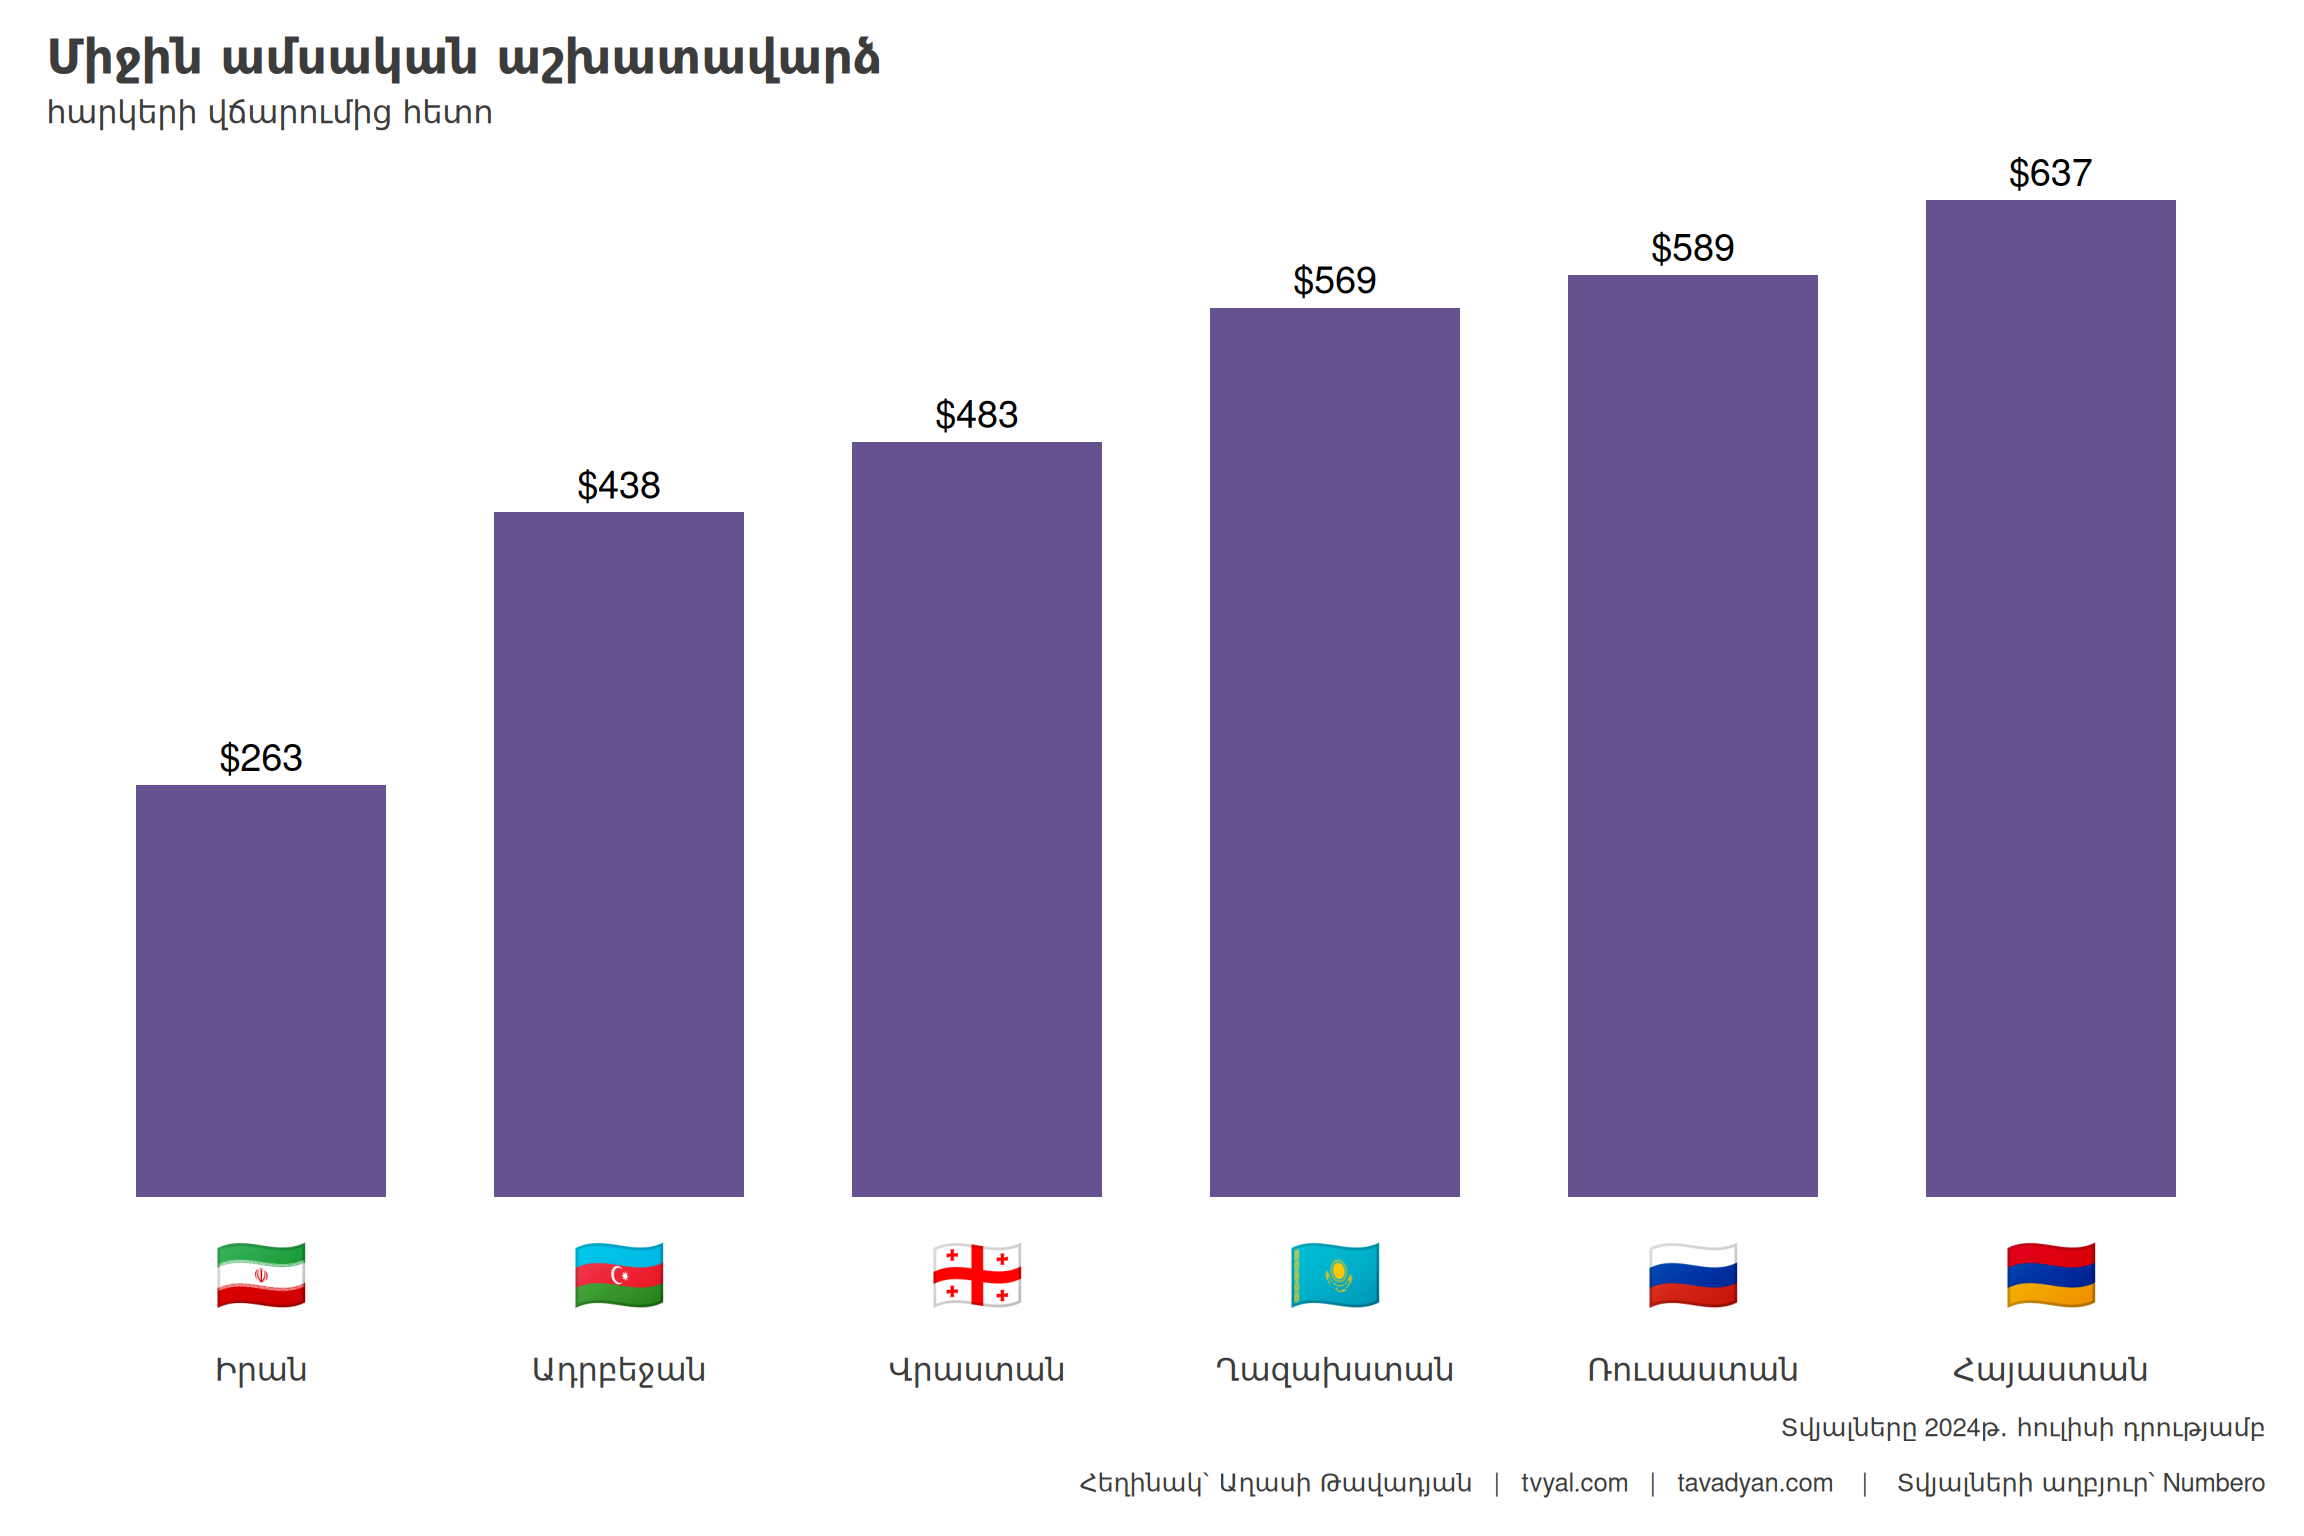
\includegraphics{TN_petrol_price_files/figure-latex/unnamed-chunk-1-1.pdf}

Գծապատկեր 2-ում ներկայացված է բենզինի ընդհանուր քանակության ներմուծումը
միլիոն կիլոգրամով: Ինչպես երևում է գծապատկերից նավթամթերքի ներմուծման
ծավալները 2010-ից 2019թ. սկիզբը եղել են գրեթե անփոփոխ: 2019 թվականից
սկսած գրանցվել է նավթամթերիքի ներմուծման շարունակական և կայուն աճ:
2017թ. ներմուծվել է համապատասխանաբար 200 և 140 մլն կիլոգրամ դիզվառելիք և
բենզին, իսկ 2022թ արդեն 300 և 225 հազար կիլոգրամ: Ընդհանուր նավթամթերի
ներկրումը վերջին 5 տարիների ընթացքում աճել է 1.5 անգամ։ Նավթամթերքը
էներգիայի կարևոր աղբյուր է, որն ապահովում է տրանսպորտային և
արդյունաբերական գործունեությունը: Երբ երկիրն ավելի շատ բենզին է
ներկրում, դա ընդհանուր առմամբ նշանակում է, որ էներգիայի ներքին
պահանջարկը մեծանում է։ Սա կարող է լինել աճող տնտեսության ցուցանիշ, որը
վկայում է սպառողական ծախսերի, ձեռնարկատիրական գործունեության և
արդյունաբերական արտադրության աճի վերաբերյալ:

\textbf{Գծապատկեր 2.} Բենզինի և դիզվառելիքի Հայաստան ներմուծման տարեկան
ծավալները

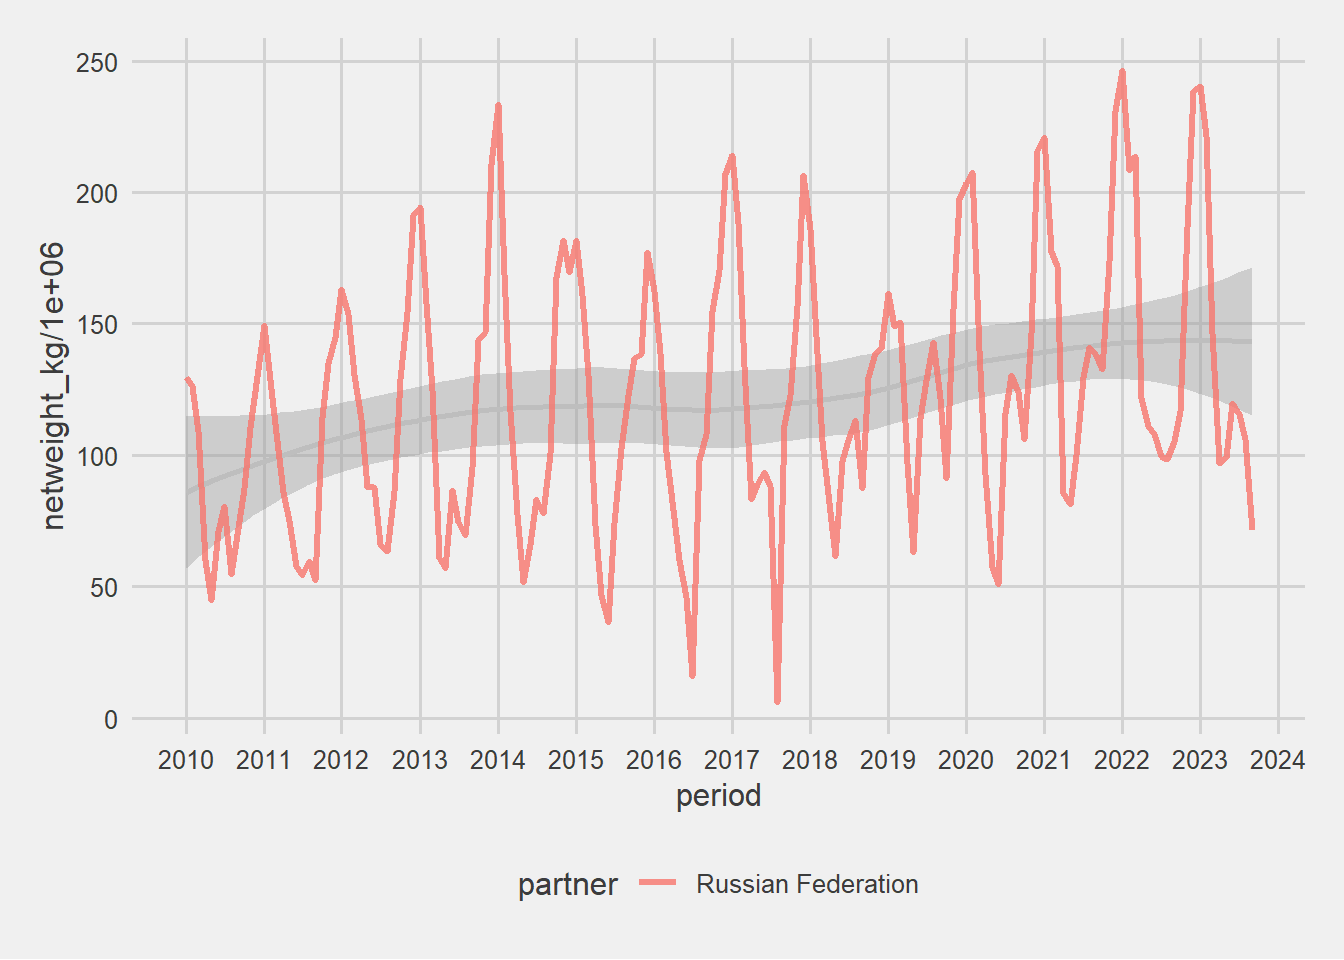
\includegraphics{TN_petrol_price_files/figure-latex/unnamed-chunk-2-1.pdf}

Գծապատկեր 3-ում ներկայացված է բենզինի գնի փոփոխությունը, ըստ 1in.am
լրատվամիջոցի օրական հրապարակումների: Այս տվյալները ստացվել են քերելով
1in.am Յութուբյան ալիքի բենզինի գների վերաբերյալ տեսանյութերի նկարները
(thumbnails): Ինչպես երևում է գծապատկերից բենզինի գինը մինչև 2023
թվականին գրանցված աճը, ամենաբարձրն է եղել 2022 թվականի ապրիլին, երբ 1
լիտր պրեմիում դասի բենզինը արժեր 540 դրամ: 2022թ. վերջին պրեմիում դասի
բենզինի գինը նվազեց մինչև 350 դրամ 1 լիտրի համար, որը գրանցվել էր 2023
թվականի փետրվարին: 2023 թվականին շարունակաբար գրանցվեց վառելիքի գնի
բարձրացում: Թե ինչո՞վ էր պայմանավորված այդ բարձրացումը կքննարկենք
հաջորդիվ:

\textbf{Գծապատկեր 3.} Բենզինի և դիզելային վառելիքի գինը Հայաստանում (ՀՀ
դրամ)

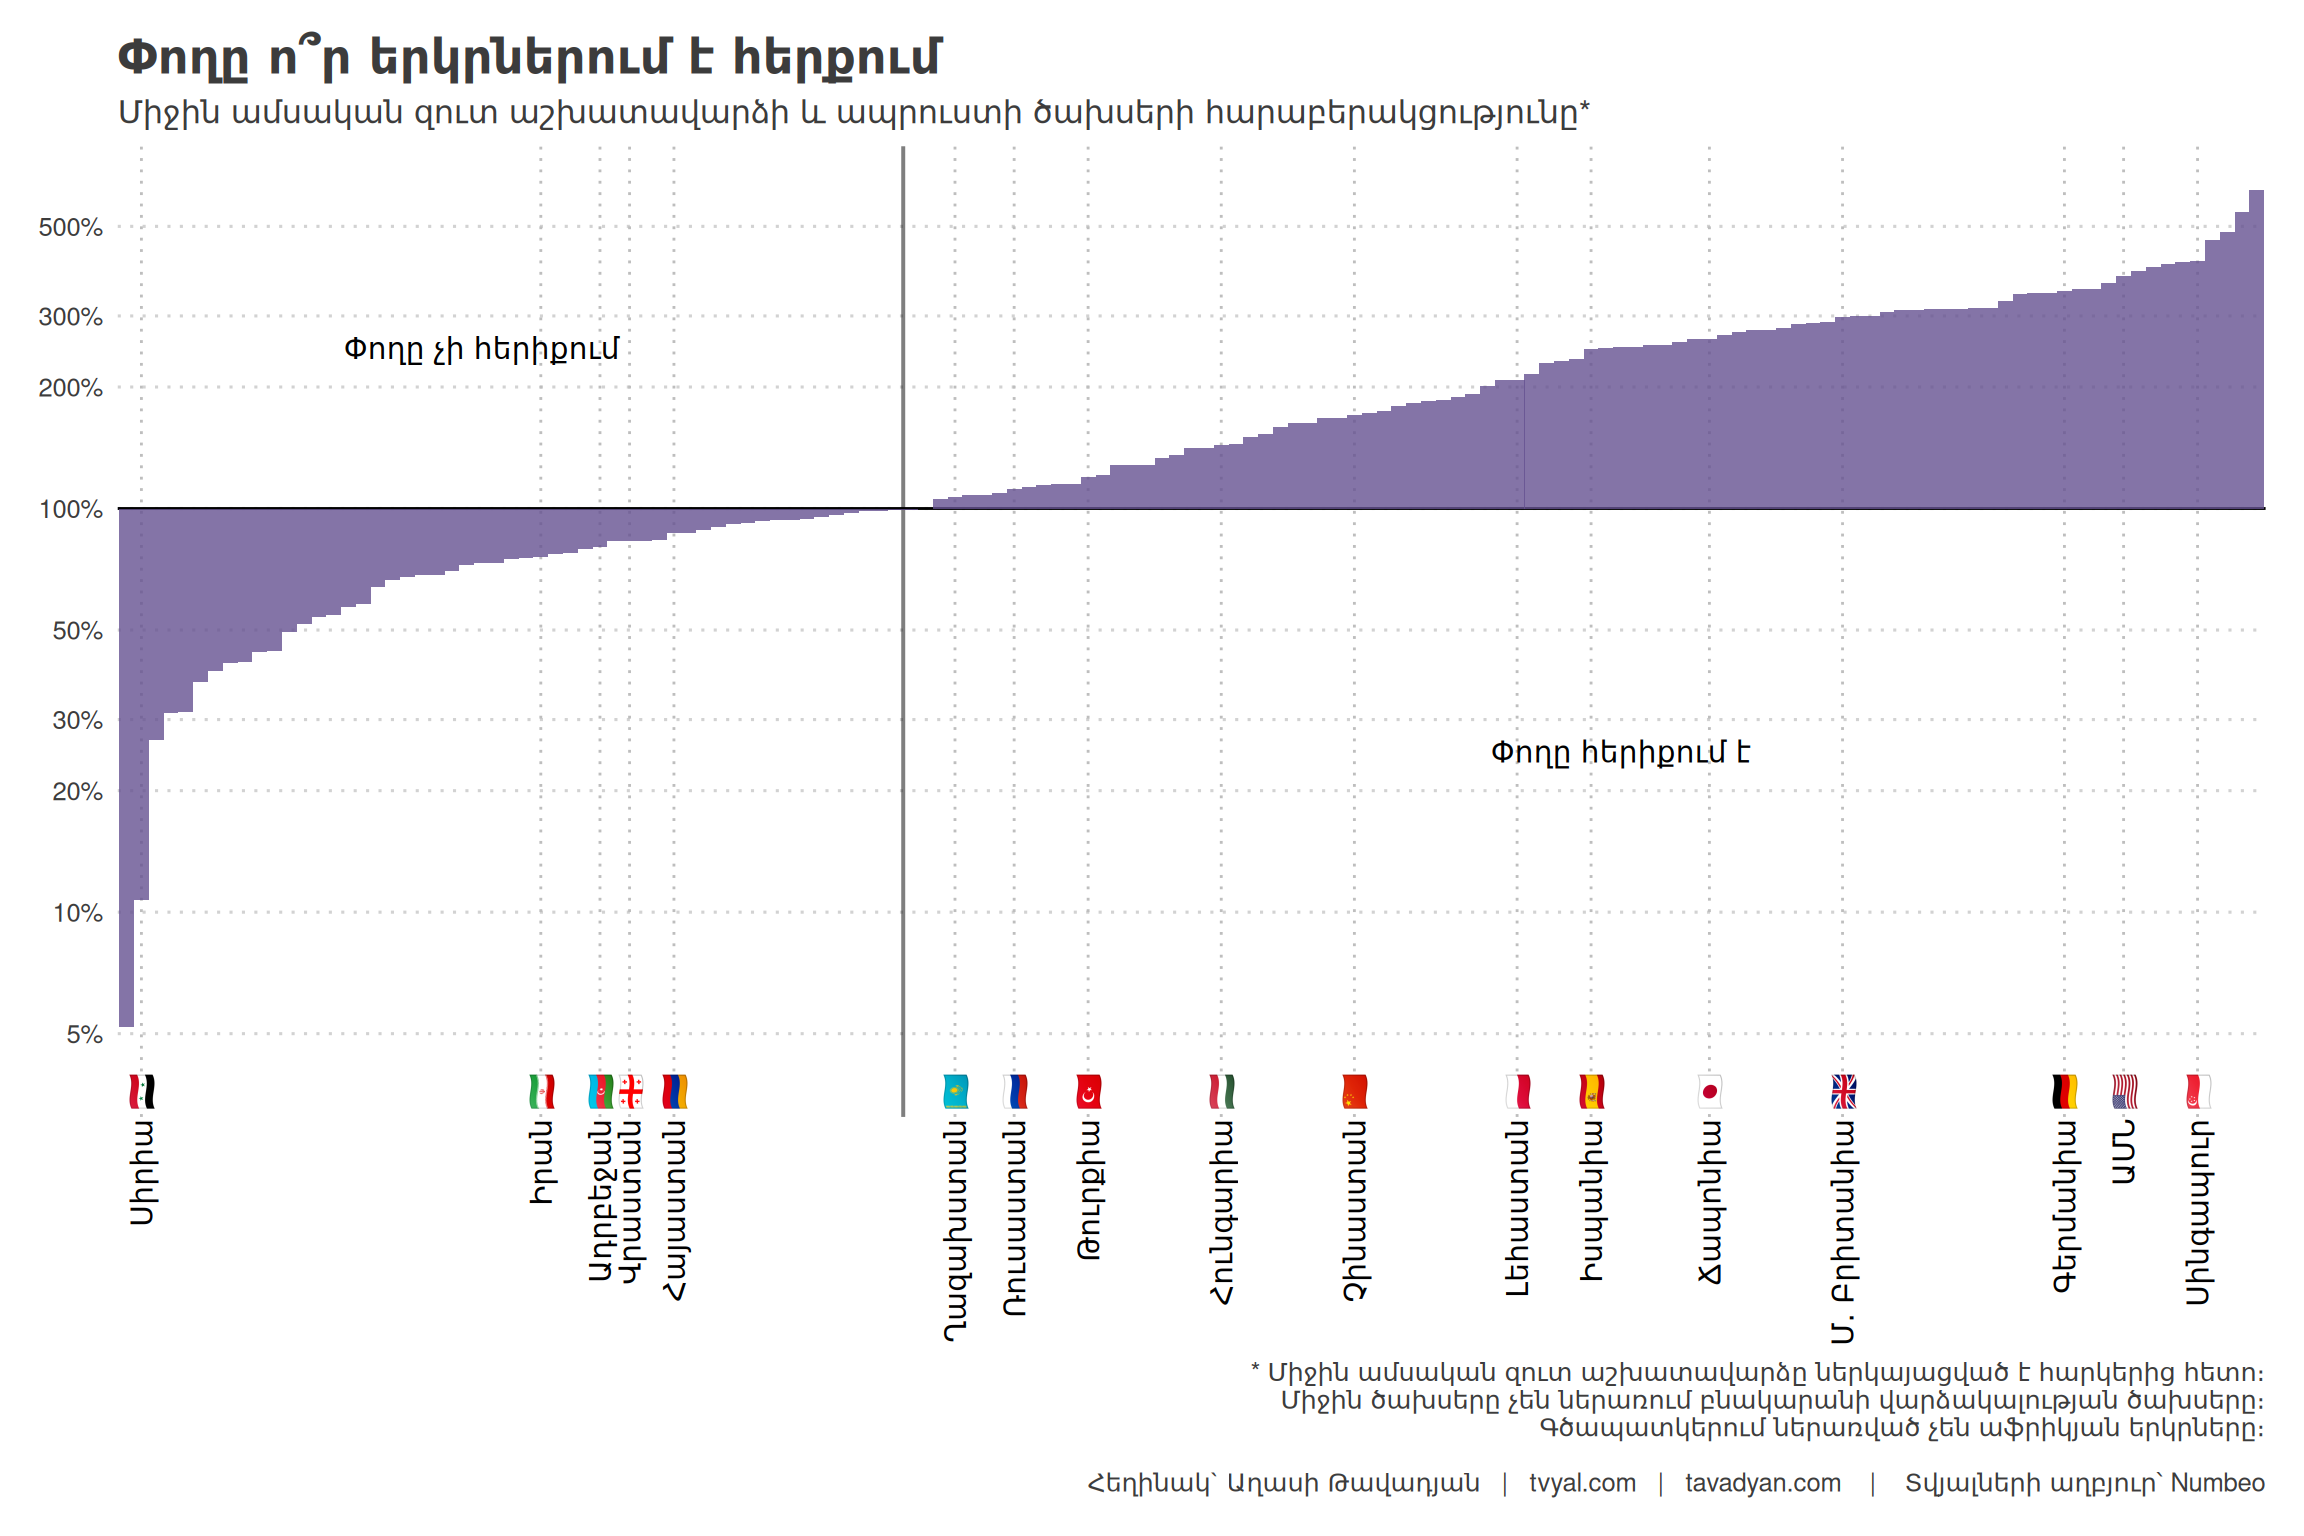
\includegraphics{TN_petrol_price_files/figure-latex/unnamed-chunk-3-1.pdf}

Հաջորդ գծապատկերում տրված է հողուկ գազի լիտրի գինը ներքին շուկայում։

\textbf{Գծապատկեր 4.} Հեղուկ գազի Հայաստանում (ՀՀ դրամ)

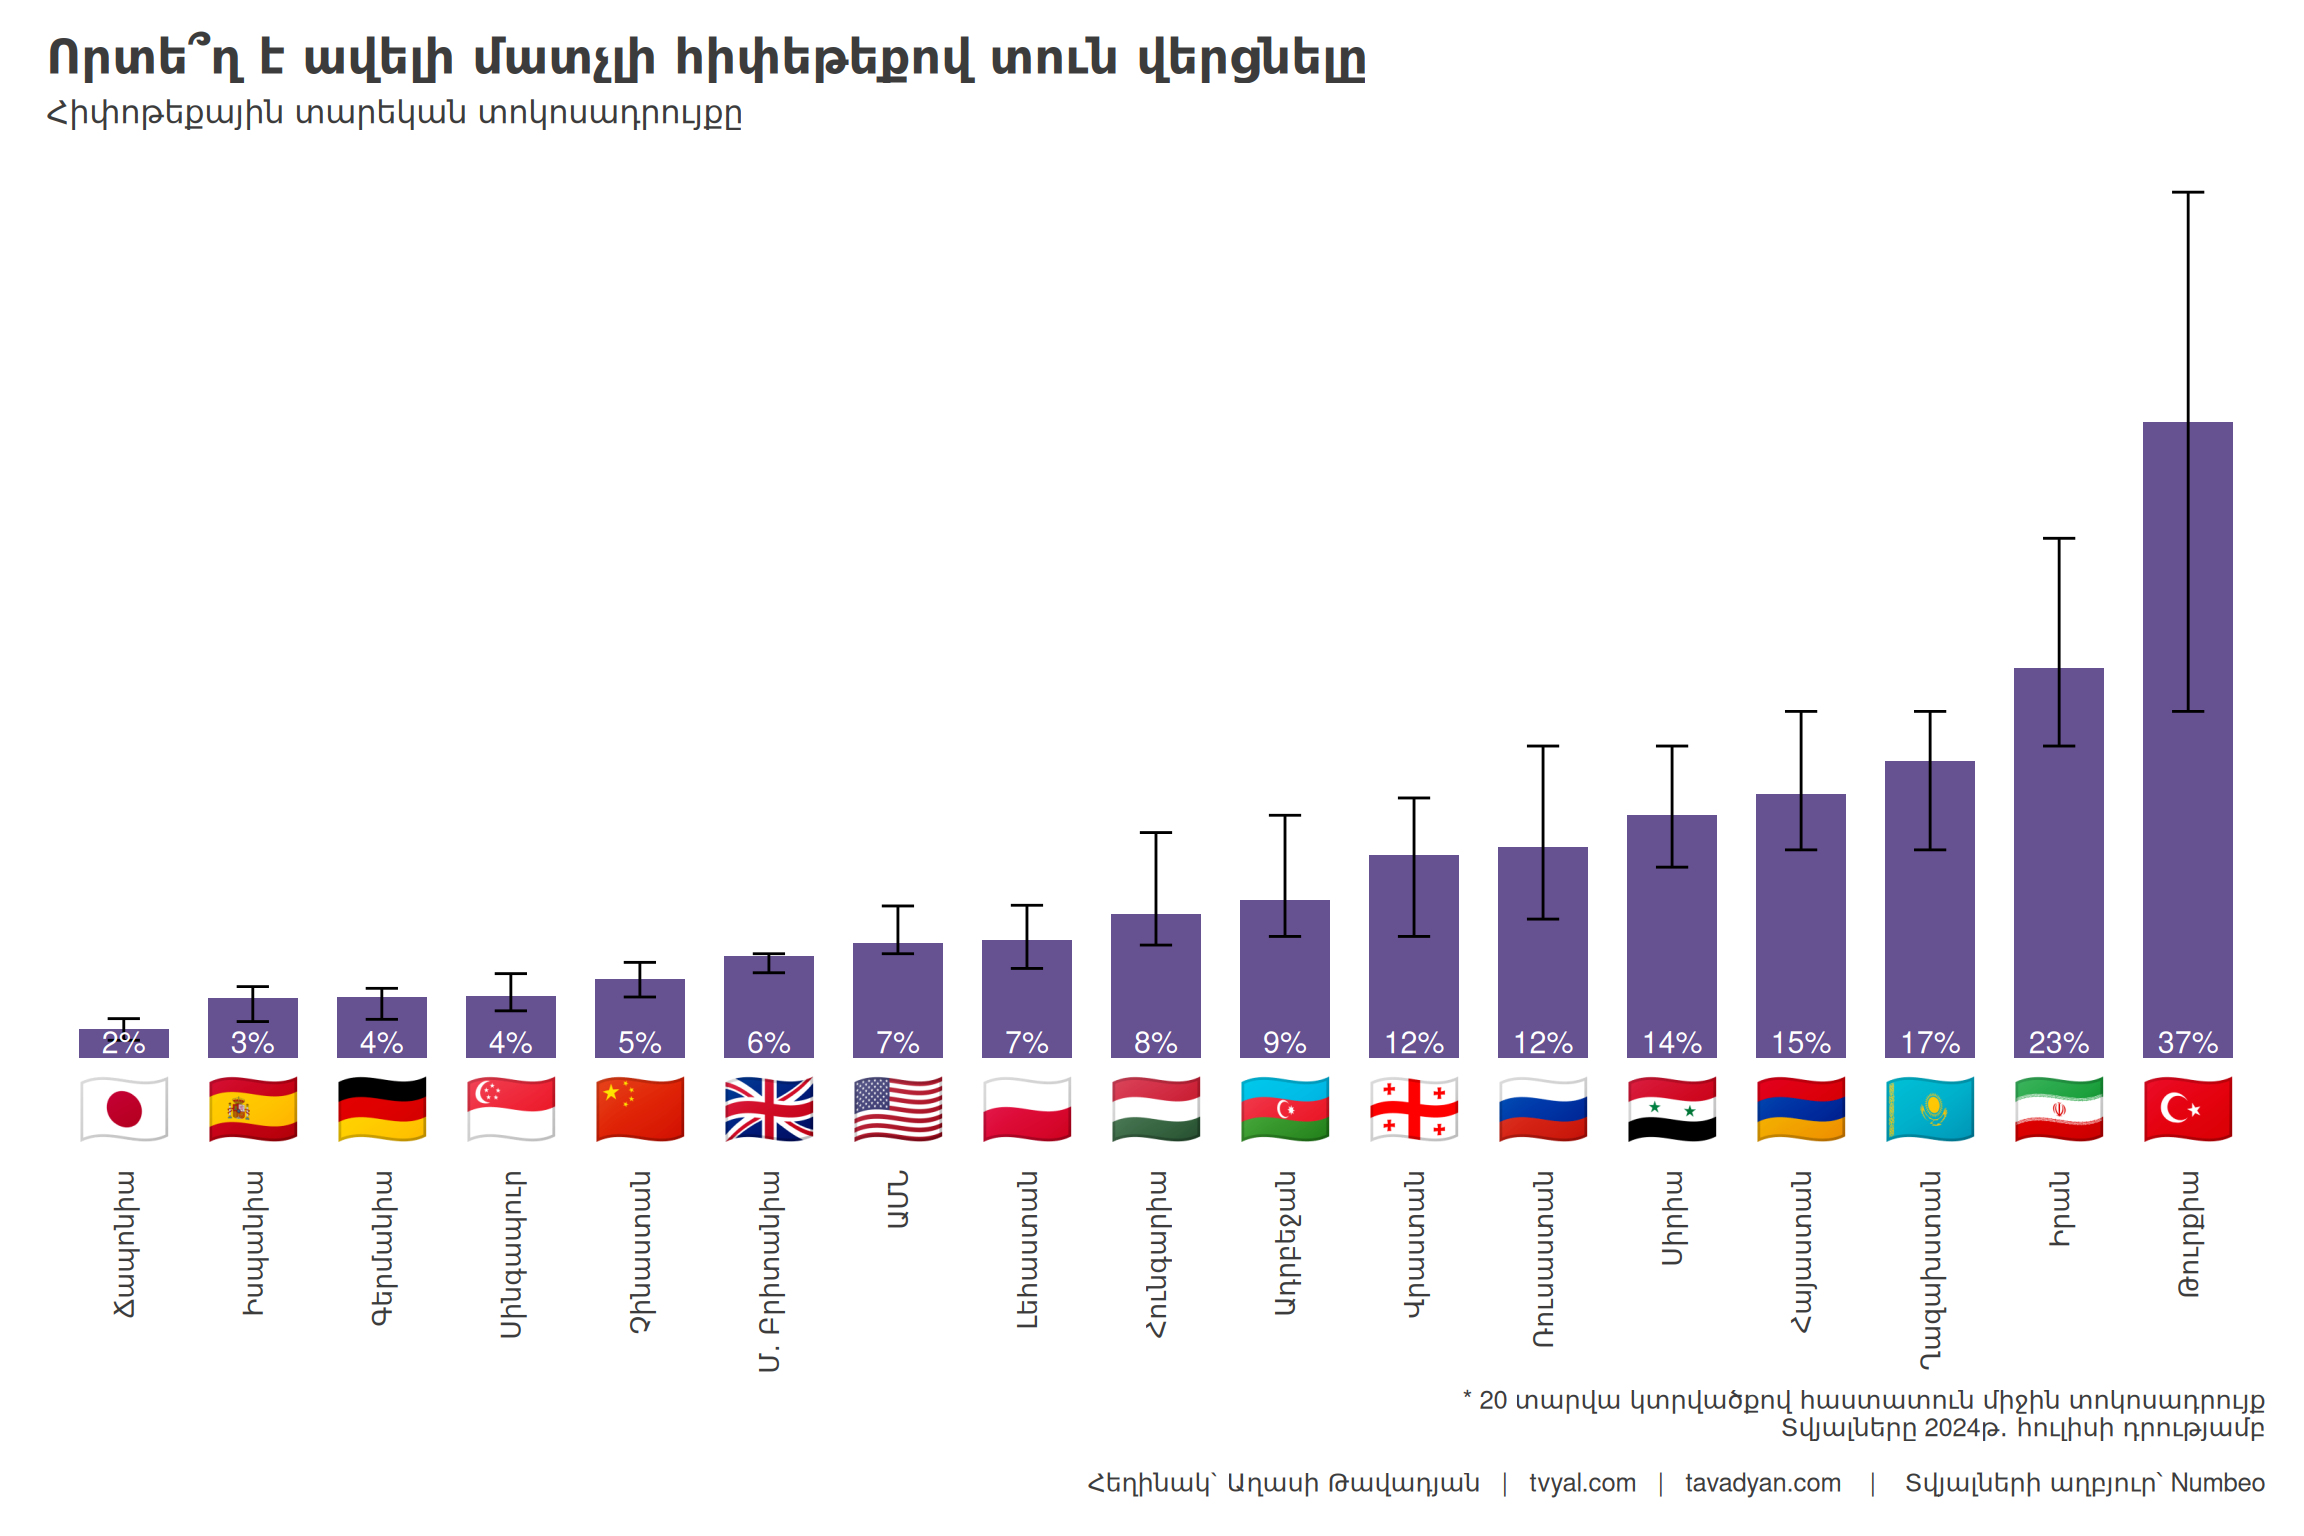
\includegraphics{TN_petrol_price_files/figure-latex/unnamed-chunk-4-1.pdf}

Ստորև ներկայացված է բենզինի և դիզելային վառելիքի ներմուծման գինը: Այն
հաշվարկվել է բաժանելով տվյալ ամսվա ներմուծման արժեքային և բնեղեն
տվյալները, որից ստացվել է բենզինի գնի կիլոգրամի ներմուծման արժեքը ԱՄՆ
դլորով: Ստացված ցուցանիշը բաժանվել է բենզինի և դիզելի խտության վրա և
բազմապատկվել տվյալ ամսվա միջին ԱՄՆ դոլար դրամ փոխարժեքով: Իհարկե ստացված
ցուցանիշը ոնի որոշակի ճշգրտության խնդիր, քանի որ նավթամթերքի խտությունը
ըստ ջերմաստիճանի կարող է փոխվել ինչպես նաև պետք է հաշվի առնել դոլարի
վաճառքի գինը ներքին շուկայում։ Սակայն այս ցուցանիշի դինամիկան հստակ
պատկերացում կարող է տալ թե ինչքանով է տարբերվում նավթամթերքի գինը
սահմանին, որը ձեռք են բերում մեր տնտեսվարողները և բենզինի գինը ներքին
շուկայում։

\textbf{Գծապատկեր 5.} Բենզինի և դեզվառելիքի ներմուծման գինը

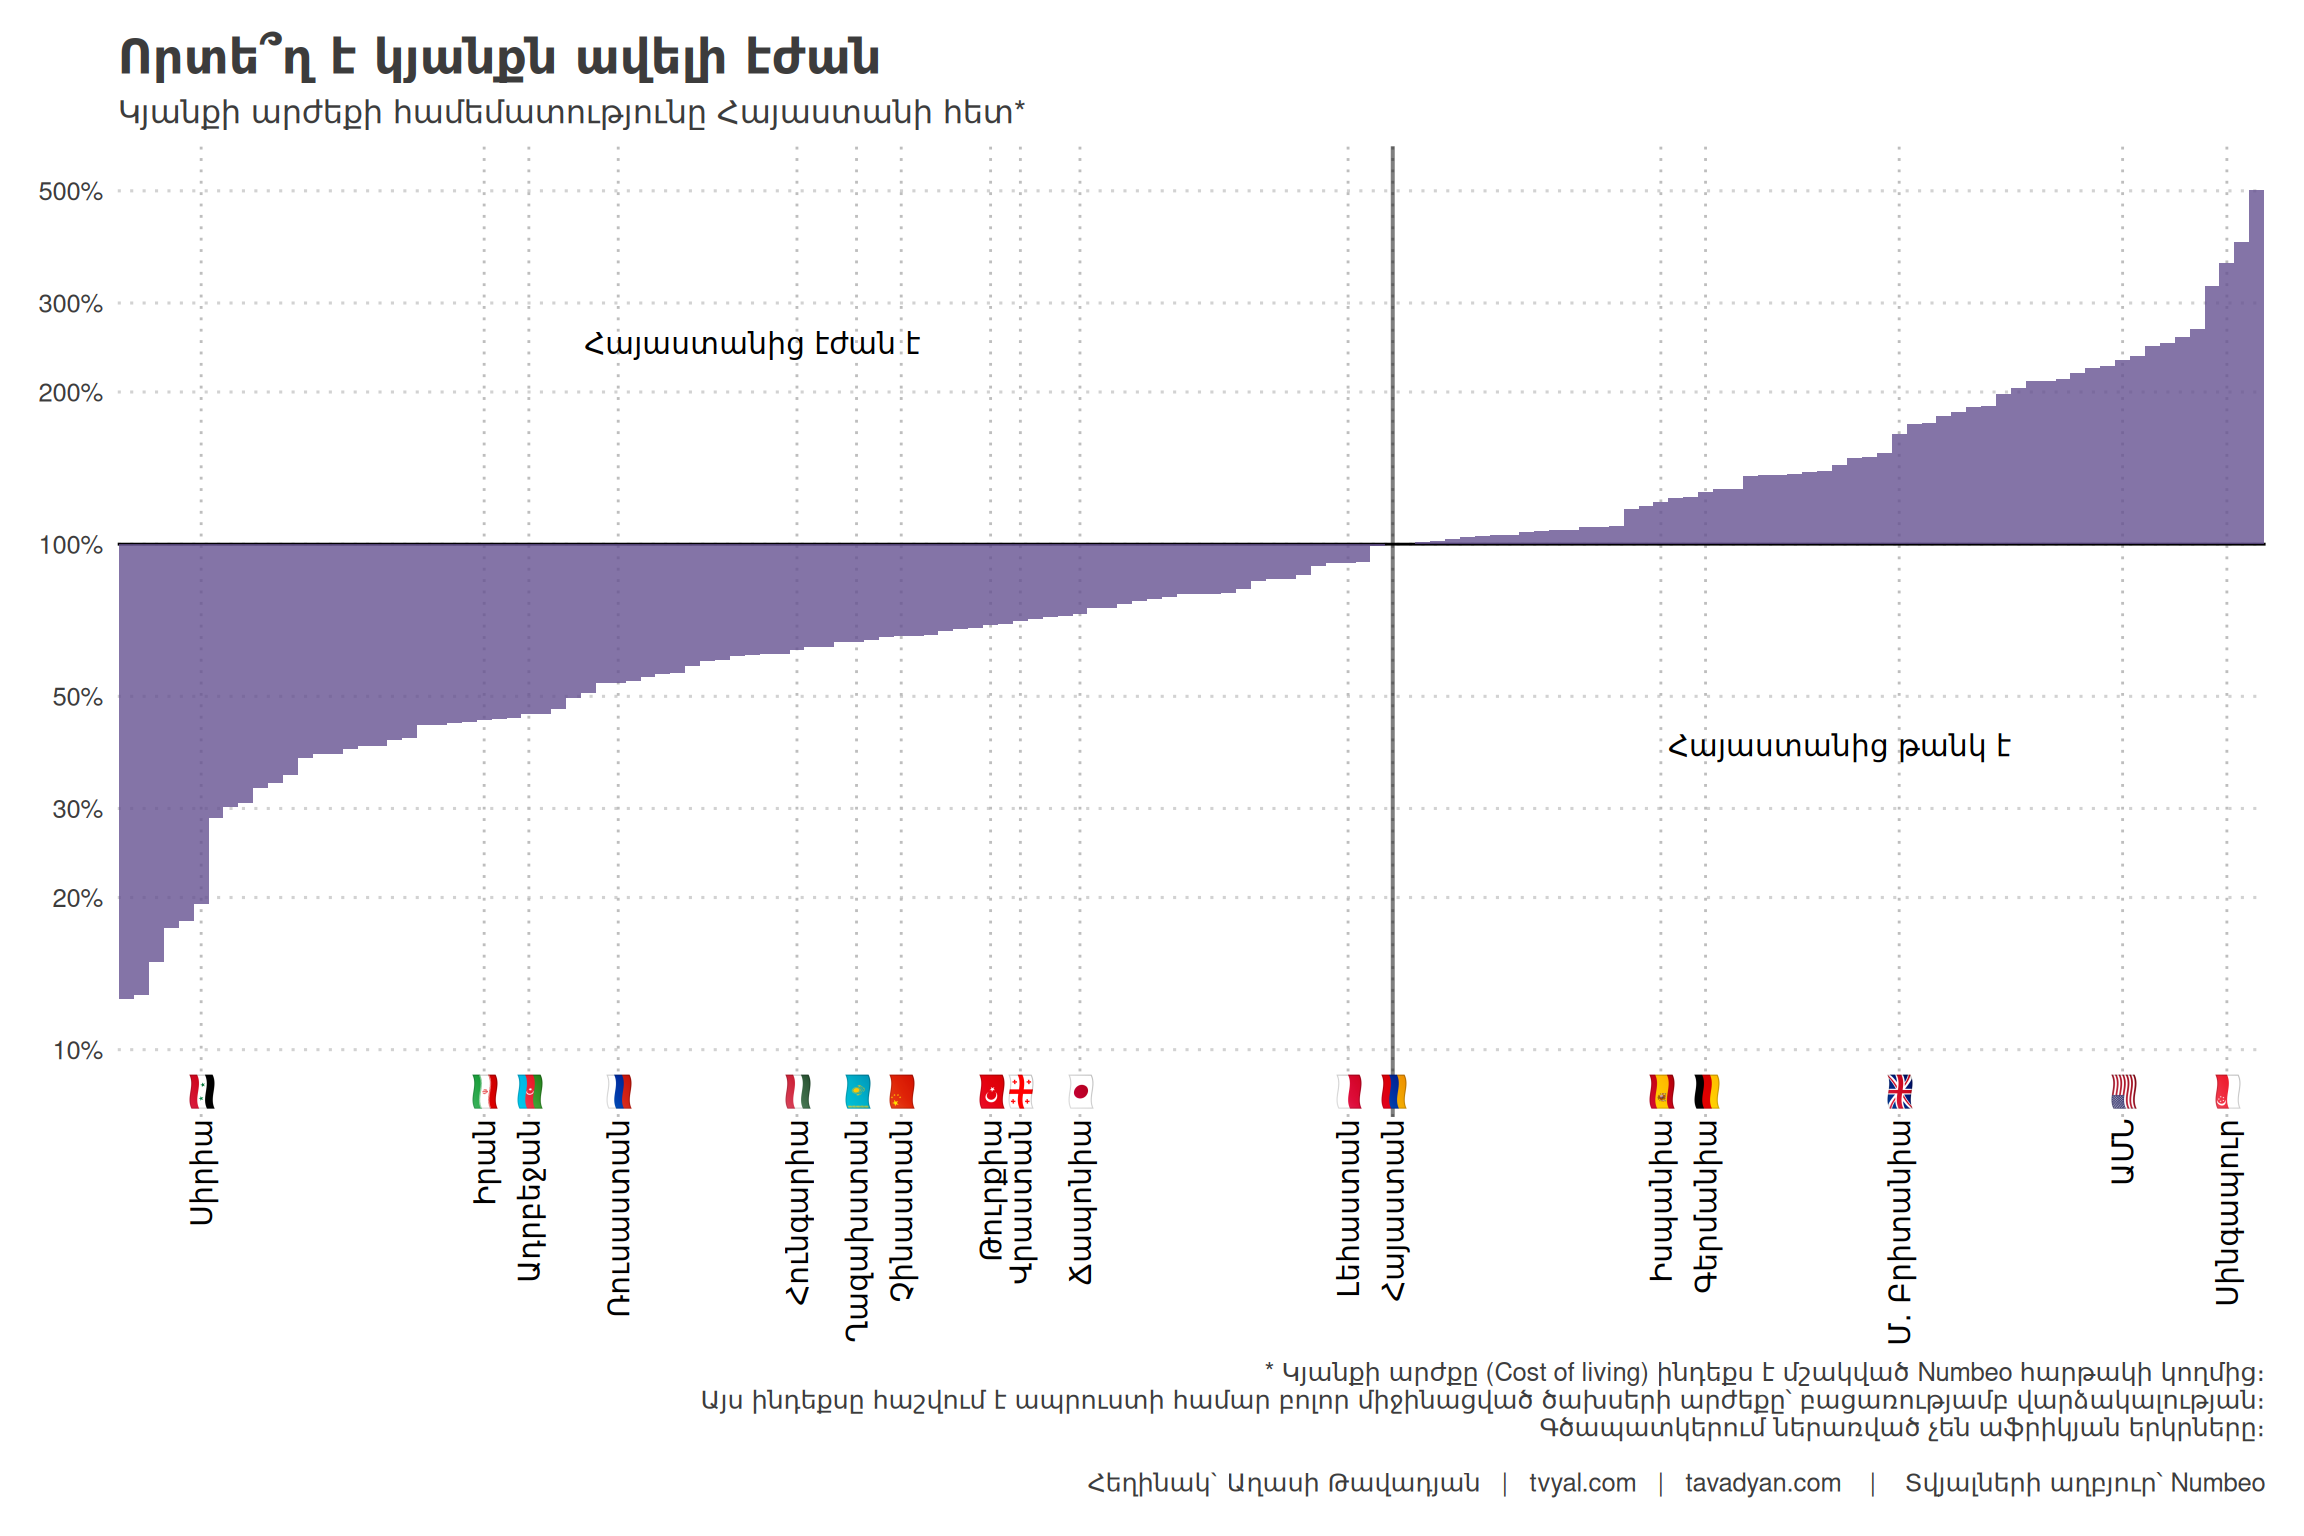
\includegraphics{TN_petrol_price_files/figure-latex/unnamed-chunk-5-1.pdf}

Դիտարկենք նաև նավթամթերքի ներմուծումը ըստ պետությունների։ Դիզելային
վառելիքը 76 տոկոսը ներմուծվում է Ռուսաստանից, 10.2 տոկոսը Իրանից:
Հետաքրքիրն այն է որ ճիշտ է Իրանի ներքին շուկայում բենզինի լիտրը շատ ցածր
գին ունի, այն Հայաստան ներմուծվում է գրեթե նույն գնով, ինչ Ռուսաստանից:
Սա կարող է քաղաքական պատճառներ ունենալ, քանի որ Ռուսաստանից եկող
նավթամթերքի գնիը թանկ է, քանի որ բարձր են տրանսպորտային ծախսերը, իսկ
Իրանի հետ մենք ունենք ուղիղ սահման:

\textbf{Գծապատկեր 6.} Բենզինի և դեզվառելիքի ներմուծման ծավալները ըստ
ծագման երկրի

\includegraphics{TN_petrol_price_files/figure-latex/unnamed-chunk-6-1.pdf}

Վերջին գծապատկերում ներկայացված է բենզինի ներմուծման գնի և շուկայական
գնի դինամիկան դիզելային վեռելիքի և բենզինի համար: Ինչպես երևում է
ներմուծման գինը և շուկայական գինը ունեն կախվածության մեծ աստիճան:
Այսինքն Հայաստանի ներքին շուկան բավականին մրցունակ է և չի կարող թելադրել
ներքին գինը։ Այն գինը ինչ սահմանին տնտեսվարողը գնում է նավթամթերը
համեմատելի է այն գնին ինչ վճարում է սովորական քաղաքացուն։

Այստեղ ներքին շուկայի գինը հաշվարկվել է ըստ սպառողական գների ինդեքսի
տվյալների բազայի, որը բազմապատկվել է 2023թ․ հոկտեմբերի վերջին գրանցված
ներքին շուկայի նավթամթերքի գներով։ Գծապատկերում ներկայացված երկու
ցուցանիշն էլ՝ գինը սհամանին և ներքին շուկայում, ունեն սխալի աստիճան։ Սա
է պատճառը որ որոշ դեպքերում բոնզինի գինը ներքին շուկայում ավելի ցածր է
քան սահմանին։ Անկախ դրանից գծապատկերը հստակ ցույց է տալիս որ նավթամթերքի
գինը սահմանին ձևավորում է գինը ներքին շուկայում։

Շուկան մրցունակ է և արագ արձագանքում է սահմանին բենզինի գների
փոփոխությանը: Բենզինի գինը կարգավորելու և այն իջեցնելու համար առաջին
հերթին այն պիտի կարգավորվի սահմանին: Հայաստանը գտնվում է ԵԱՏՄ ընդհանուր
շուկայում և ըստ ԵԱՏՄ համաձայնագրի պետք է գործի ընդհանուր
էներգառեսուրսների շուկա: Բենզինի գնի համեմատաբար բարձր լինելը
հիմնականում պայմանավորված է տրանսպորտային ծախսերով: Հնարավոր է բենզինի
ներմուծումը դիվերսիֆիկացնել և այն ներմուծել Իրանից, որտեղից
տրանսպորտային ծախսերը ավելի քիչ կլինեն, սակայն սա արդեն քաղաքատնտեսական
և ներ ենթակառուցվածքների ձևավովորման հարց է։

\textbf{Գծապատկեր 7.} Նավթամթերքի ներմուծաման և շուկայական գնի
տարբերությունը

\includegraphics{TN_petrol_price_files/figure-latex/unnamed-chunk-7-1.pdf}

\hypertarget{ux566ux56cux574-ux570ux561ux572ux578ux580ux564ux561ux563ux580ux578ux582ux569ux575ux578ux582ux576ux576ux565ux580}{%
\subsection{2. ԶԼՄ
հաղորդագրություններ}\label{ux566ux56cux574-ux570ux561ux572ux578ux580ux564ux561ux563ux580ux578ux582ux569ux575ux578ux582ux576ux576ux565ux580}}

\href{https://www.youtube.com/watch?v=59NRXzTdMqY}{Factor.tv}
լրատվամիջոցով խոսել եմ նրա մասին թե ի՞նչ ազդեցություն ունի Ռուսաստանը
Հայաստանի տնտեսության վրա։ Հարցազրույցը ռուսերենով է:

\href{https://www.youtube.com/watch?v=59NRXzTdMqY}{\includegraphics{https://i3.ytimg.com/vi/59NRXzTdMqY/maxresdefault.jpg}}

\href{https://www.panorama.am/am/news/2023/11/17/\%D4\%B1\%D5\%B2\%D5\%A1\%D5\%BD\%D5\%AB-\%D4\%B9\%D5\%A1\%D5\%BE\%D5\%A1\%D5\%A4\%D5\%B5\%D5\%A1\%D5\%B6/2927178}{Panorama}
լրատվամիջոցին տվել եմ հարցազրույց բենզինի գնի մասին, թե ինչպես է այն
ձևավորվում մեր շուկայում։

\href{https://www.youtube.com/watch?v=zwQu5vD5yCg}{\includegraphics{https://i3.ytimg.com/vi/zwQu5vD5yCg/maxresdefault.jpg}}

\hypertarget{ux57dux57aux561ux57dux578ux582ux574-ux565ux574-ux571ux565ux566-ux56bux574-ux57dux569ux580ux56bux574ux56bux576}{%
\subsection{3. Սպասում եմ ձեզ իմ
սթրիմին}\label{ux57dux57aux561ux57dux578ux582ux574-ux565ux574-ux571ux565ux566-ux56bux574-ux57dux569ux580ux56bux574ux56bux576}}

Եթե ձեզ հետաքրքիր է լսել իմ մեկնաբանությունները և տեսնել թե ոնց եմ ես
կատարում իմ հետազոտությունները, կարող եք մասնակցել իմ սթրիմին։

\href{https://www.facebook.com/events/1125123785538008/}{}

Ես նպաստակադրված եմ այն ամենը ինչ անում եմ ներկայացնել և բացատրել սթրիմի
կամ վլոգի ձևաչափով: Սա նախնական և փորձնական է լինելու, որը հոսով եմ
շարունակական կլինի։

\hypertarget{english-summary}{%
\subsection{4. English Summary}\label{english-summary}}

\textbf{Exploring Gasoline Prices -- What's Behind the Recent Spike?}

This week's newsletter delves into the factors influencing the recent
surge in gasoline prices in Armenia. It analyzes various data sources,
including daily petrol and diesel price data, monthly fuel price
databases, and fuel import statistics. Highlighting Armenia's position
as a significant gasoline-importing country, the analysis explores the
impact of transportation costs and Armenia's non-oil-producing status on
fuel prices. It notes the steady increase in petroleum product imports
since 2019 and discusses the correlation between gasoline prices, import
volumes, and domestic demand for energy. The newsletter emphasizes the
competitive nature of Armenia's domestic oil market and suggests that
regulating prices at the border is crucial for effectively managing and
lowering gasoline prices in the country. The potential to diversify
gasoline imports from Iran as a means of reducing transportation costs
is also explored as a possible solution. The comprehensive data
visualizations accompanying the analysis provide a detailed overview of
the key trends and dynamics driving gasoline prices in Armenia.

Այս վերլուծությունը առկա է նաև
\href{https://www.tvyal.com/newsletter/2023_11_20}{մեր կայքէջում}, այս
վերլուծության կոդը և տվյալները դրված են նաև
\href{https://github.com/tavad/tvyal_newsletter}{Github-ում}։

Եթե հնարավոր է, խնդրում եմ այս նյութը ուղարկել նաև այն մարդկանց, ում այն
կարծում եք կարող է հետաքրքրել:

Սպասեք հաջորդ հաղորդագրությանը մի շաբաթվա ընթացքում:

Հարգանքներով,\\
Աղասի Թավադյան\\
21.11.2023\\
\href{https://www.tvyal.com/}{tvyal.com}\\
\href{https://www.tavadyan.com/}{tavadyan.com}

\textbf{Ուշադրություն. Ձեր էլ.փոստը մեյլիսթի մեջ է, որի միջոցով ես
կիսվում եմ շաբաթական նյութեր, որոնք հիմնականում ներկայացնում են
Հայաստանի տնտեսությանը: Նյութերը ներառում են գծապատկերներ,
\href{https://github.com/tavad/tvyal_newsletter}{տվյալների բազաներ},
տեսանյութեր, հոդվածներ, \href{https://www.tvyal.com/projects}{առցանց
վահանակներ}, տնտեսական գործիքներ, կանխատեսումներ և հաշվետվություններ:
Եթե ցանկանում եք չեղարկել բաժանորդագրությունը, խնդրում եմ տեղեկացրեք
ինձ, և ես կհեռացնեմ ձեր էլ. փոստը ցուցակից: Գրեք նաև եթե ունեք
մենկնաբանություններ:}

\textbf{Important! Your email is part of the mailing list where I share
weekly materials primarily focused on the Armenian economy. These
materials encompass charts,
\href{https://github.com/tavad/tvyal_newsletter}{databases}, videos,
articles, \href{https://www.tvyal.com/projects}{online dashboards},
economic tools, forecasts, and reports. If you wish to unsubscribe,
please let me know, and I will remove your email from the list. Please
share your comments as well․}

\end{document}
